\section{Refinamento diádico adaptativo certificado}
O refinamento usa majorantes locais validados de $|F''|$ para controlar o erro em cada célula.

\subsection{Fechamento operacional por aritmética intervalar}
Seja $\EE$ a menor classe de expressões que contém $x$ e as constantes racionais e é fechada por soma, subtração, produto, recíproco, $\exp$, $\sin$, $\cos$ e composição. Um recíproco é admissível em intervalos nos quais seu denominador não se anula. Essa classe contém os polinômios, as funções racionais sem polos no domínio e as funções elementares usadas nos exemplos.

Composição significa substituição sintática: em $u\circ v$, cada folha $x$ da árvore de $u$ é substituída pela árvore de $v$. Toda expressão composta é, assim, uma árvore das operações-base.

Escreva $\mathbb I_{\Q}$ para os intervalos fechados com extremos racionais. A rotina
\eqn{36}{\operatorname{BoundSecondDerivative}(E,J;P,d)
=[\underline m_J,\overline m_J]\in\mathbb I_{\Q}}
usa precisão transcendental $P$ e profundidade de subdivisão $d$. Ela propaga simultaneamente intervalos para $(E,E',E'')$, isto é, 2-jatos intervalares. Por exemplo,
\begin{align*}
(uv)''&=u''v+2u'v'+uv'',\\
(u^{-1})''&=2(u')^2u^{-3}-u''u^{-2},\\
(e^u)''&=e^u\bigl((u')^2+u''\bigr),\\
(\sin u)''&=-\sin(u)(u')^2+\cos(u)u'',\\
(\cos u)''&=-\cos(u)(u')^2-\sin(u)u''.
\end{align*}
As operações racionais são exatas. Para $\exp$, a redução do argumento a $|z|\le1/2$ é seguida por uma soma de Taylor com resto majorado por uma série geométrica racional; para $\sin$ e $\cos$, usa-se o resto de Lagrange racional e a interseção com $[-1,1]$. Elevar $P$ e $d$ reduz a sobrestimação.

\begin{lema}[restos transcendentais com extremos racionais]
Se $I=[a,b]\in\mathbb I_{\Q}$, as rotinas descritas acima produzem intervalos de extremos racionais que contêm $\exp(I)$, $\sin(I)$ e $\cos(I)$. Mais explicitamente, para $0\le z\le1/2$ e $n\ge0$,
\eqn{37}{0\le e^z-\sum_{j=0}^n\frac{z^j}{j!}
\le\frac{z^{n+1}}{(n+1)!}\frac1{1-z/(n+2)}.}
Se $R=\max\{|a|,|b|\}$ e
\[
P_n^{\sin}(z)=\sum_{j=0}^n(-1)^j\frac{z^{2j+1}}{(2j+1)!},\qquad
P_n^{\cos}(z)=\sum_{j=0}^n(-1)^j\frac{z^{2j}}{(2j)!},
\]
então, para todo $z\in I$,
\eqn{38}{|\sin z-P_n^{\sin}(z)|\le\frac{R^{2n+2}}{(2n+2)!},\qquad
|\cos z-P_n^{\cos}(z)|\le\frac{R^{2n+1}}{(2n+1)!}.}
Avaliar os polinômios em $I$, inflar pelos respectivos restos e intersectar com $[-1,1]$ preserva a inclusão.
\end{lema}
\begin{proof}
Na série de $e^z$, o primeiro termo omitido é $t_{n+1}=z^{n+1}/(n+1)!$. Para $j\ge n+1$, a razão entre termos consecutivos é $z/(j+1)\le z/(n+2)<1$; a cauda é, portanto, majorada pela série geométrica de primeiro termo $t_{n+1}$ e razão $z/(n+2)$, o que dá \eqref{eq:37}. Para um argumento racional $x$ arbitrário, escolha $r$ com $z=|x|/2^r\le1/2$, aplique a inclusão anterior e eleve o intervalo ao quadrado $r$ vezes; se $x<0$, tome o recíproco do intervalo positivo obtido para $-x$. Em $I=[a,b]$, a monotonicidade de $e^x$ permite usar o extremo inferior da inclusão em $a$ e o superior da inclusão em $b$.

As duas desigualdades em \eqref{eq:38} são o resto de Lagrange dos polinômios de Maclaurin de graus $2n+1$ e $2n$, pois todas as derivadas de seno e cosseno têm módulo no máximo $1$. A avaliação intervalar contém a imagem de cada polinômio; inflar pelo raio do resto contém a função. Como seno e cosseno já pertencem a $[-1,1]$, a interseção não remove nenhum valor possível. Todas as operações, fatoriais e extremos envolvidos são racionais.
\end{proof}

\begin{proposicao}[correção do majorante intervalar]
Se $E\in\EE$ define uma função $C^2$ em $J$ e a rotina \eqref{eq:36} termina com sucesso, então
\eqn{39}{E''(x)\in[\underline m_J,\overline m_J]\ (x\in J),\qquad
M_{\rm int}(J):=\max\{|\underline m_J|,|\overline m_J|\}\ge\normK{E''}{J}.}
Se algum intervalo de denominador contém zero mesmo após a subdivisão permitida, a rotina devolve falha e nenhum número é aceito como certificado.
\end{proposicao}
\begin{proof}
Para constantes e para $x$, a inclusão é imediata. Soma, produto e recíproco preservam inclusão pelas operações elementares de intervalos; o recíproco só é executado quando zero está fora do intervalo do denominador. As fórmulas de 2-jatos acima e o lema~6.1 dão o passo de indução estrutural para toda expressão de $\EE$. Pela normalização sintática declarada antes do lema, uma composição genérica já foi expandida nessa árvore e não acrescenta um caso independente. Subdividir $J$ preserva a cobertura, e tomar o fecho convexo dos intervalos obtidos em suas partes contém a união das imagens de $E''$. Isso prova a primeira inclusão e, tomando módulos, \eqref{eq:39}. A regra de falha impede que uma divisão não validada produza uma falsa garantia.
\end{proof}
A propagação registra a largura dos intervalos, o número de caixas e a profundidade usados. Subdivisão e Taylor racional permitem apertar as inclusões.

\begin{algoritmo}[refinamento certificado]
Dados $f\in C^2[\alpha,\beta]$, tolerâncias $\varepsilon_I,\varepsilon_R>0$ e a extensão $F$ de \eqref{eq:30}, use, para toda célula $J$, um majorante validado
\eqn{40}{\normK{F''}{J}\le M(J)\le M_*<\infty.}
Quando $F$ é fornecida por uma expressão de $\EE$, tome $M(J)=M_{\rm int}(J)$ de \eqref{eq:39}; se a certificação falhar, aborte sem emitir uma montagem garantida. Para uma função $C^2$ fora dessa interface, \eqref{eq:40} é um contrato de entrada.
\begin{enumerate}[label=(\roman*),topsep=6pt,itemsep=3pt]
\item Inicie com uma cobertura diádica finita de $[\alpha,\beta]$.
\item Para cada folha $J$, calcule
\eqn{41}{\eta_{\rm cert}(J)=\frac{|J|^2M(J)}8.}
\item Enquanto existir folha com $\eta_{\rm cert}(J)>\varepsilon_I$, substitua-a por seus dois filhos.
\item Nos nós finais, escolha racionais compartilhados $v_t$ com $|v_t-F(t)|<\varepsilon_R$ e valores adjacentes distintos.
\item Emita, em cada folha, o endereço do átomo que interpola seus dois valores nodais.
\end{enumerate}
\end{algoritmo}

\begin{teorema}[correção, término e tamanho]
O algoritmo~6.3 termina e produz $g\in\Asm([\alpha,\beta])$ com
\eqn{42}{\norm{f-g}\le\varepsilon_I+\varepsilon_R.}
Se a cobertura inicial tem $R_0$ raízes de largura máxima $h_0$ e $M_*>0$, nenhuma ramificação ultrapassa
\eqn{43}{r_*=\max\left\{0,\left\lceil\frac12\log_2\left(\frac{h_0^2M_*}{8\varepsilon_I}\right)\right\rceil\right\}}
níveis, e há no máximo $R_02^{r_*}$ folhas. Se $M_*=0$, pode-se tomar $r_*=0$.
\end{teorema}
\begin{proof}
Após $r$ subdivisões, uma folha descendente de uma raiz tem $|J|\le h_02^{-r}$ e, por \eqref{eq:40},
\[
\eta_{\rm cert}(J)\le\frac{h_0^2M_*}8\,4^{-r}.
\]
O lado direito é no máximo $\varepsilon_I$ para $r\ge r_*$; logo nenhuma folha é subdividida além dessa profundidade. A árvore é finita e cada raiz gera no máximo $2^{r_*}$ folhas.

Na partição final, \eqref{eq:34} e \eqref{eq:40} implicam
\[
\normK{F-P_\Lambda F}{J}\le\frac{|J|^2}8\normK{F''}{J}\le\eta_{\rm cert}(J)\le\varepsilon_I.
\]
A racionalização nodal produz, pelos teoremas~3.5 e 3.6, uma montagem de átomos de endereço único e com $\norm{P_\Lambda F-g}<\varepsilon_R$. Como $F=f$ no intervalo original, a desigualdade triangular prova \eqref{eq:42}.
\end{proof}
\begin{figure}[H]\centering
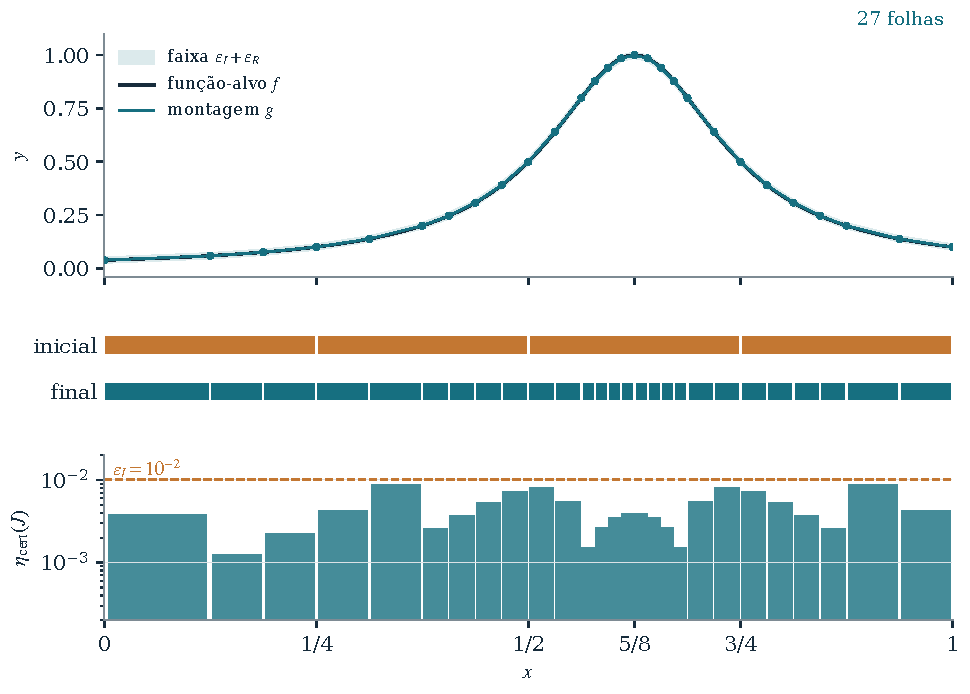
\includegraphics[width=.90\linewidth]{figuras/06_refinamento_certificado.pdf}
\caption{Refinamento certificado para $f(x)=[1+64(x-5/8)^2]^{-1}$. Células com certificado acima de $\varepsilon_I$ são subdivididas. A malha se concentra na região de maior curvatura, e o painel inferior compara os certificados finais com a tolerância. A faixa superior representa o limite uniforme $\varepsilon_I+\varepsilon_R$.}
\label{fig:refinamento}
\end{figure}

\begin{proposicao}[calibração exata para curvatura constante]
Suponha que $[\alpha,\beta]=J_0$ seja uma única célula diádica inicial, $F''\equiv\kappa\ne0$ em $J_0$ e $M(J)=|\kappa|$ em todo descendente. Pondo
\[
A=\frac{|J_0|^2|\kappa|}8,
\]
o número de folhas produzido com tolerância $\varepsilon_I$ é
\eqn{44}{N(\varepsilon_I)=2^{r(\varepsilon_I)},\qquad
r(\varepsilon_I)=\max\left\{0,\left\lceil\log_4\left(\frac A{\varepsilon_I}\right)\right\rceil\right\}.}
Consequentemente,
\eqn{45}{\begin{aligned}
\liminf_{\varepsilon_I\downarrow0}\sqrt{\varepsilon_I}\,N(\varepsilon_I)
&=\frac1{\sqrt8}\int_\alpha^\beta|f''(x)|^{1/2}\,dx,\\
\limsup_{\varepsilon_I\downarrow0}\sqrt{\varepsilon_I}\,N(\varepsilon_I)
&=\frac1{\sqrt2}\int_\alpha^\beta|f''(x)|^{1/2}\,dx.
\end{aligned}}
A quantização diádica introduz, nesse caso, um fator dois entre os limites de acumulação.
\end{proposicao}
\begin{proof}
Após $r$ subdivisões uniformes, cada folha tem largura $|J_0|2^{-r}$ e certificado $A4^{-r}$. Como todos os certificados de um mesmo nível são iguais, o algoritmo para no primeiro $r$ com $A4^{-r}\le\varepsilon_I$, o que prova \eqref{eq:44}. Para $A4^{-r}\le\varepsilon_I<A4^{-(r-1)}$, tem-se
\[
\sqrt A\le\sqrt{\varepsilon_I}\,2^r<2\sqrt A.
\]
Os extremos inferior e superior são atingidos, respectivamente, nos limiares $\varepsilon_I=A4^{-r}$ e por aproximação pela esquerda aos limiares $A4^{-(r-1)}$. Por fim, $\int_\alpha^\beta|f''|^{1/2}=|J_0|\sqrt{|\kappa|}$.
\end{proof}

\begin{observacao}[diferença segunda e erro no centro]
Se $x_0=(x_L+x_R)/2$, então
\[
|f(x_0)-P_Jf(x_0)|=\frac12|f(x_L)-2f(x_0)+f(x_R)|.
\]
Isso mede o erro no centro. Para $f(x)=x^3$ em $[-1,1]$, $P_Jf(x)=x$ e a diferença segunda central é zero, enquanto
\[
\norm{x^3-x}=\frac2{3\sqrt3}\approx0{,}3849.
\]
O controle em todo o intervalo é fornecido pelo majorante de \eqref{eq:40}.
\end{observacao}
